\chapter{Introducere}

\section{Context}
Aceasta secțiune descrie contextul lucrării și motivele care au condus la necesitatea dezvoltării acestei cercetări. În ultimii ani, criptomonedele și tehnologia blockchain au înregistrat o creștere exponențială, devenind nu doar mijloace de investiție, ci și instrumente valoroase pentru inovare în diverse domenii, inclusiv educația digitală. Platformele care recompensează utilizatorii cu criptojetoane au apărut ca o soluție inovatoare în acest spațiu, oferind nu doar oportunități de învățare, ci și de câștig prin implicare activă.

În acest context economic și tehnologic, a apărut necesitatea explorării modului în care aceste platforme pot fi extinse pentru a acoperi un spectru mai larg de subiecte educaționale, dincolo de sfera criptomonedelor și a blockchain-ului. Această lucrare își propune să investigheze potențialul și viabilitatea dezvoltării unei platforme educaționale de tip learn-to-earn care să recompenseze utilizatorii pentru participarea la cursuri din domenii variate, în special cele din sfera STEM (Știință, Tehnologie, Inginerie și Matematică).

\begin{figure}[H]
    \centering
    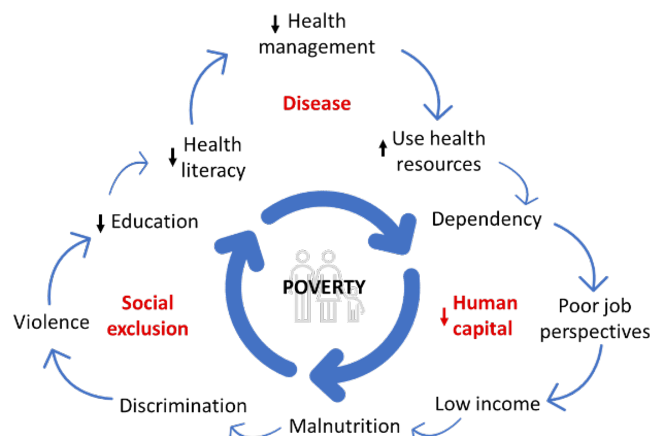
\includegraphics[width=\textwidth]{Figuri/The-impacts-from-the-vicious-circle-of-poverty.png}
    \caption{Impacturile din cercul vicios al sărăciei.\protect\footnotemark}
    \label{fig:cerc_vicios_saracie}
\end{figure}
\footnotetext{Sursa: Bell, Victoria et al., "Community Health of Children and Adolescents in Sub-Saharan Africa", European Journal of Medical and Health Sciences, 2023. DOI:10.24018/ejmed.2023.5.3.1702.}




Figura \ref{fig:cerc_vicios_saracie} ilustrează ``cercul vicios al sărăciei'', evidențiind cum diverse aspecte negative ale vieții socio-economice și de sănătate sunt legate între ele, formând un cerc vicios. Asta înseamnă că problemele precum sărăcia, malnutriția, lipsa de educație și sănătatea precară se influențează și se întăresc una pe alta. De exemplu, sărăcia poate duce la o alimentație slabă, care afectează sănătatea, iar o sănătate precară poate împiedica o persoană să muncească și să câștige bani, ceea ce menține sărăcia. Aceste probleme sunt atât de strâns legate încât este greu să le rezolvi separat; trebuie să le abordezi pe toate pentru a rupe acest cerc vicios.


\subsection{Motivație}
Motivația pentru această cercetare derivă din necesitatea de a depăși limitările platformelor existente și de a explora modalități noi și eficiente de a stimula învățarea într-un cadru mai larg, care să integreze domenii diverse din educația STEM. Prin extinderea aplicabilității recompenselor cu criptojetoane la o gamă variată de subiecte educaționale, această cercetare propune o abordare inovatoare care poate contribui la democratizarea accesului la educație de calitate și la creșterea interesului pentru domeniile STEM.

\subsection{Cum o platformă educațională bazată pe criptojetoane ar putea contribui la spargerea acestui ciclu vicios}

O platformă educațională care recompensează utilizatorii cu criptojetoane pentru finalizarea cursurilor și pentru implicarea activă ar putea aborda mai multe dintre elementele negative prezentate în figura \ref{fig:cerc_vicios_saracie}:

\begin{itemize}
    \item \textbf{Accesul la educație}: Sărăcia reduce accesul la educație, care la rândul său menține indivizii într-un cerc de excludere socială și oportunități limitate de angajare. O platformă care oferă acces gratuit sau la costuri reduse la cursuri online, recompensându-i pe utilizatori cu criptojetoane, ar putea crește accesul la educație, în special în regiunile defavorizate. Aceasta ar putea contribui la îmbunătățirea alfabetizării și a competențelor profesionale, sporind astfel șansele de angajare și veniturile.
    
    \item \textbf{Creșterea capitalului uman}: Sărăcia duce la o scădere a capitalului uman, reducând astfel șansele de a obține locuri de muncă bine plătite și de a ieși din sărăcie. Prin stimularea învățării și dezvoltării competențelor, platforma ar putea contribui la creșterea capitalului uman, oferind astfel utilizatorilor posibilitatea de a accesa joburi mai bine plătite sau de a iniția proiecte antreprenoriale. Recompensele în criptojetoane ar putea fi utilizate fie pentru investiții suplimentare în educație, fie pentru îmbunătățirea condițiilor de viață.
    
    \item \textbf{Îmbunătățirea sănătății și a gestionării acesteia}: Sărăcia și educația deficitară duc la o sănătate precară și la o gestionare ineficientă a resurselor de sănătate, ceea ce perpetuează starea de sărăcie. Platforma ar putea oferi cursuri de educație pentru sănătate, igienă și nutriție, contribuind astfel la creșterea alfabetizării în domeniul sănătății. Utilizatorii ar putea învăța cum să își gestioneze mai bine sănătatea și resursele, reducând astfel incidența bolilor și dependența de servicii de sănătate costisitoare.
    
    \item \textbf{Reducerea excluziunii sociale}: Sărăcia este adesea însoțită de excluderea socială și discriminare, care reduc șansele indivizilor de a participa activ în societate. Platforma poate construi o comunitate globală de învățare, în care utilizatorii să interacționeze, să colaboreze și să se sprijine reciproc, reducând astfel excluderea socială. Recompensele în criptojetoane pot oferi recunoaștere și stimulente pentru participarea activă, consolidând sentimentul de apartenență și valoare personală.
\end{itemize}

\subsection{Lucrări înrudite}
În literatura de specialitate și în practica curentă, există diverse platforme de tip learn-to-earn, cum ar fi BitDegree \cite{bitdegree} și Phemex Learn Crypto \cite{phemex}, care recompensează utilizatorii pentru finalizarea cursurilor online. Acestea se concentrează în principal pe subiecte legate de criptomonede și tehnologia blockchain. Cu toate acestea, aceste platforme au o limitare semnificativă: restrângerea domeniului de aplicabilitate la teme crypto, fără a acoperi un spectru mai larg din domeniul STEM. Astfel, cercetarea de față propune o extindere a acestui model de recompensare către domenii educaționale mai diversificate, contribuind la o mai bună integrare a acestor tehnologii în educația generală.

% Adaugă alte secțiuni/subsecțiuni după nevoie